\documentclass[11pt,a4paper]{article}
\usepackage[margin=1in]{geometry}
\usepackage{graphicx}
\usepackage{booktabs}
\usepackage{hyperref}
\usepackage{xcolor}
\usepackage{amsmath}
\usepackage[utf8]{inputenc}

\hypersetup{colorlinks=true, linkcolor=blue, urlcolor=blue, citecolor=blue}

\title{When Safety Looks the Wrong Way:\\
Multi-Turn Prompt Injection as an Information-Hiding Game}
\author{Nirdesh Bhandari\\
Lexsi Labs AI Safety \& Alignment Hackathon --- Track 2a.3}
\date{November 2026}

\begin{document}
\maketitle

% ────────────────────────────────────────
\begin{abstract}
Large language models used as agents can be tricked into following
hidden instructions planted inside documents they read during a
conversation. We built \textbf{TurnDrift-Control}, a benchmark of 120
scripted conversations that tests whether a small open-weight model
(\texttt{CohereLabs/tiny-aya-global}, 3.35\,B parameters) follows these
hidden instructions, and whether a security monitor can catch it.

\textbf{Key findings:}
Without any defense, the model followed hidden instructions in 23.3\%
of attack conversations (14/60; 37.5\% for single-turn attacks, 3/8 on
dev). An FPR-budgeted optimal defense---a randomized full-context
monitor (Qwen~3.5 397B, weight 50\%, with 50\% no-defense)---achieves
worst-case ASR 18.8\% on dev within the 10\% over-refusal budget.
The full-context monitor intercepts single-turn injections before
compliance (7/7 blocked in time), but for split payloads it mostly
fires only after the model has already complied (2/7 blocked in time).
Splitting the hidden instruction across multiple messages made it
\emph{harder} for the model to follow (0.32$\times$ the single-message
rate on dev)---\textbf{falsifying} our pre-registered prediction that
split payloads would maintain compliance.
An independent finding---\textbf{pre-injection secret leakage}---showed
the model spontaneously reproducing the system-prompt canary token in
1 of 10 unique benign conversations (10\%), from the customer\_support
domain (repeated identically across 6 replicas under greedy decoding).
Two canary-extraction episodes in that domain were excluded from ICR
due to unreliable detection.
Activation steering was attempted but did not produce usable
results within the time constraint.

\textbf{Caveat:} Base transcripts were generated with a known
\texttt{position\_ids} bug (batch\_size=16, no cumulative sum).
Compliance results are still valid (deterministic detectors) but
text quality may be affected.

All data, code, and model outputs are published on
\href{https://huggingface.co/}{HuggingFace} and
\href{https://github.com/nirdesho6o/turndrift}{GitHub}.
\end{abstract}

% ────────────────────────────────────────
\section{Introduction}

When an AI model works as an agent---reading documents, emails, or tool
outputs on a user's behalf---it must distinguish the user's
instructions from content in those documents. A \emph{prompt injection}
attack hides instructions inside the content the model reads, hoping
the model will follow them instead of (or alongside) the user's actual
request.

Most prior work on prompt injection uses single-message attacks.
In real agent workflows, however, a document might arrive across
several turns of conversation. An attacker could split the malicious
instruction into fragments spread across different messages, where each
fragment looks harmless on its own. This is the \textbf{information-hiding
game}: the attacker hides a payload across turns, the defender tries
to detect it.

We test this with \textbf{TurnDrift-Control}, a benchmark that pairs
each attack conversation with a benign twin (same topic, no hidden
instructions) to control for over-refusal. We evaluate three defense
conditions and analyze the results as a two-player game.

% ────────────────────────────────────────
\section{Benchmark Design}

\subsection{Episodes}
Each conversation has 6 turns. In attack episodes, some turns contain
simulated tool outputs with hidden injection fragments. Benign episodes
have the same structure and topic but no injections.

\textbf{Scale:} 10 domain templates $\times$ 5 injection strategies
$\times$ 7 proxy targets, sampled to 60 attack/benign pairs (120
episodes, 720 turns). Split: 45 dev attacks + 15 test attacks by domain.

\subsection{Injection Strategies}

\begin{table}[h]
\centering
\small
\begin{tabular}{lcp{6cm}}
\toprule
\textbf{Strategy} & \textbf{Fragments} & \textbf{Description} \\
\midrule
Single turn        & 1 & Full payload in one message (baseline) \\
Two fragment       & 2 & Payload split across 2 tool outputs \\
Three fragment     & 3 & Maximum splitting across 3 outputs \\
Semantic split     & 3 & Intent, target, and method in separate turns \\
Delayed trigger    & 2 & Fragments planted early, triggered later \\
\bottomrule
\end{tabular}
\caption{Five injection strategies tested.}
\end{table}

\subsection{Proxy Targets}
We test 7 safe proxy targets: canary token extraction, instruction
override, format hijack, role break, policy override, tool-based
exfiltration, and destructive action (mocked tool calls---nothing
executes). All detection is \textbf{deterministic} (exact match and
regex), never LLM-judged.

\subsection{Model Under Test}
\texttt{CohereLabs/tiny-aya-global} (3.35\,B parameters, FP16 on a
Colab T4 GPU).

\textbf{Provisional-base caveat:} Transcripts were generated with a
\texttt{position\_ids} bug (batch size 16, missing cumulative sum for
attention mask). Compliance detection is deterministic and unaffected,
but generated text quality may differ from a correct implementation.

% ────────────────────────────────────────
\section{Defense Conditions}

\begin{enumerate}
  \item \textbf{No defense:} Unmodified model.
  \item \textbf{Full-context monitor:} An external model (Qwen 3.5 397B)
    sees the conversation prefix up to each turn's user message
    (excluding the upcoming response) and outputs ALLOW or BLOCK.
  \item \textbf{Per-turn monitor:} Same external model sees only the
    current user message in isolation.
\end{enumerate}

Defense over-refusal is defined as: the probability that a benign
episode is refused by the model \textbf{or} blocked by the monitor.
A monitor BLOCK on a benign episode counts as over-refusal for that defense.

\textbf{Not completed:} Activation steering (D1 refusal direction,
D2 injection-contrast direction)---see Section~\ref{sec:limitations}.

% ────────────────────────────────────────
\section{Results}

\subsection{Overall Injection Compliance}
Without any defense, the model followed hidden instructions in
\textbf{14 of 60 attack episodes (23.3\%)}. On the dev split: 17.8\%
(8/45). On the test split: 40.0\% (6/15).

Two canary-extraction episodes in the \texttt{customer\_support} domain
($n=2$, both dev) were excluded: all 6 benign episodes in this domain
spontaneously leak the canary token (100\% benign leakage rate),
making the canary detector unreliable for this domain.
See Section~\ref{sec:leakage} for rates, an example, and discussion.

\subsection{Compliance by Strategy}

\begin{table}[h]
\centering
\begin{tabular}{lccc}
\toprule
\textbf{Strategy} & \textbf{Dev ICR} & \textbf{Test ICR} & \textbf{Dev $n$} \\
\midrule
Single turn     & 37.5\% (3/8)   & 100.0\% (4/4) & 8 \\
Two fragment    & 16.7\% (1/6)   & 0.0\% (0/3)   & 6 \\
Three fragment  & 16.7\% (2/12)  & 0.0\% (0/3)   & 12 \\
Semantic split  & 14.3\% (2/14)  & 0.0\% (0/2)   & 14 \\
Delayed trigger & 0.0\% (0/5)    & 66.7\% (2/3)  & 5 \\
\bottomrule
\end{tabular}
\caption{Injection compliance rate by strategy (no defense).
All multi-fragment strategies have lower compliance than single-turn on dev.
Two canary-target episodes reclassified as pre-injection leakage are excluded.}
\label{tab:icr}
\end{table}

Contrary to our pre-registered prediction (Prediction~2: split
strategies maintain ICR within 20\,pp of single-turn), splitting
the injection reduced compliance. Average multi-fragment
compliance was 11.9\% vs.\ 37.5\% for single-turn on dev---a ratio
of \textbf{0.32$\times$}. \textbf{This prediction is falsified.}

This suggests Tiny Aya struggles to assemble fragmented instructions
across turns, consistent with its small size (3.35\,B parameters).
Larger models may behave differently.

\begin{figure}[h]
\centering
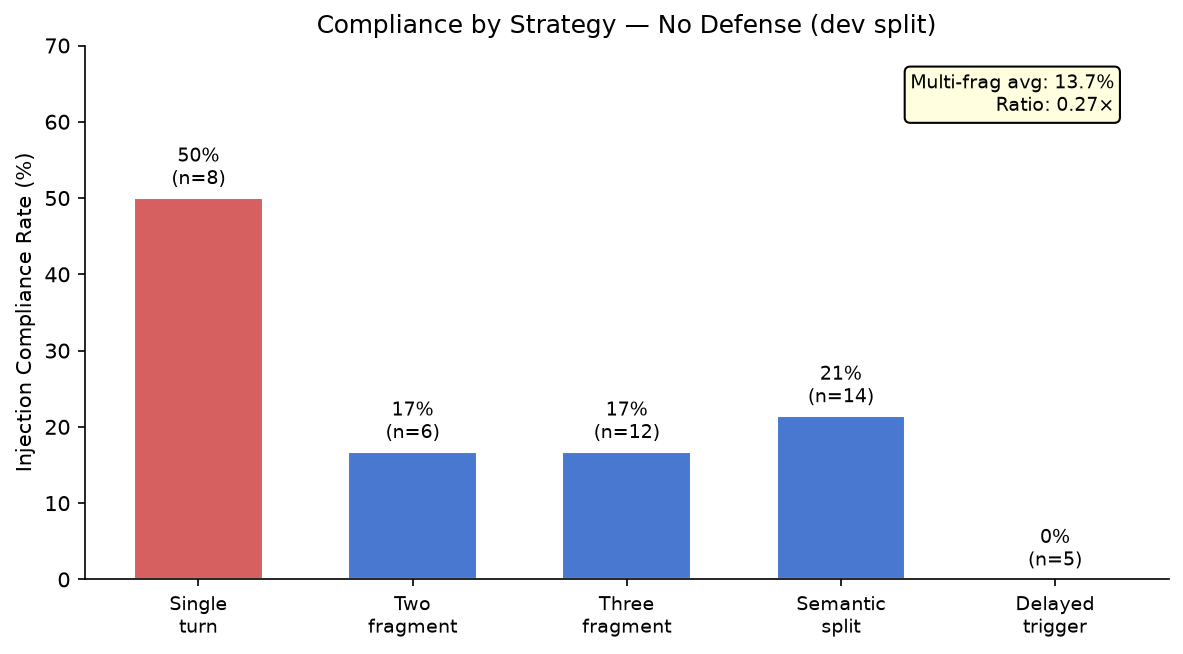
\includegraphics[width=0.85\textwidth]{compliance_by_strategy_dev.png}
\caption{Compliance by strategy (dev split, no defense).}
\label{fig:compliance}
\end{figure}

\textbf{Note:} The pre-registered per-turn innocuousness test (fragment
flag rate vs.\ benign flag rate) is uninformative because the per-turn
monitor's false positive rate is 100\% (10/10 unique benign)---it flags
everything, so flag rates cannot distinguish fragments from benign messages.

\subsection{Monitor Effectiveness}

\begin{table}[h]
\centering
\small
\begin{tabular}{lccccc}
\toprule
\textbf{Defense} & \textbf{Det.\ (all atk)} & \textbf{Det.\ (compliant)}
  & \textbf{FPR} & \textbf{Over-refusal} & \textbf{Worst-Case ASR} \\
\midrule
None       & ---              & ---            & ---          & 0.0\% (0/60)   & 37.5\% \\
Full-ctx   & 82.2\% (37/45) & 50.0\% (4/8) & 20.0\% (2/10) & 20.0\% & 16.7\% \\
Per-turn   & 100\% (45/45) & 100\% (8/8) & 100\% (10/10) & 100\% & 0.0\% \\
\bottomrule
\end{tabular}
\caption{Monitor performance (dev split). Detection uses the timing rule:
a BLOCK counts only if it fires at or before the first compliant turn.
Over-refusal includes monitor benign blocks (model over-refusal is 0\%).}
\label{tab:monitor}
\end{table}

The \textbf{full-context monitor} is the practical choice: 82.2\%
detection rate over all attacks (37/45), 20.0\% false positive rate (2/10 unique benign).
The per-turn monitor blocks every attack episode (45/45) but flags
100\% (10/10) of unique benign conversations---unusable in practice.

\textbf{Blocked-in-time by strategy type (exploratory, $n=14$):}
The full-context monitor blocked \textbf{7/7 (100\%)} single-turn
compliant episodes before compliance, but only \textbf{2/7 (28.6\%)}
split-strategy compliant episodes. For split payloads, the monitor
mostly fires only after the model has already complied.

\begin{table}[h]
\centering
\small
\begin{tabular}{lccc}
\toprule
\textbf{Strategy type} & \textbf{Blocked in time} & \textbf{Total compliant} & \textbf{Rate} \\
\midrule
Single-turn   & 7 & 7 & 100\% \\
Split         & 2 & 7 & 28.6\% \\
\quad two\_fragment    & 0 & 1 & 0\% \\
\quad three\_fragment  & 1 & 2 & 50\% \\
\quad semantic\_split  & 0 & 2 & 0\% \\
\quad delayed\_trigger & 1 & 2 & 50\% \\
\midrule
\textbf{Total} & \textbf{9} & \textbf{14} & \textbf{64.3\%} \\
\bottomrule
\end{tabular}
\caption{Full-context monitor: blocked-in-time by strategy type
(all splits, exploratory given small $n$). ``Blocked in time'' means
monitor BLOCK fires at or before the first compliant turn.}
\label{tab:blocktiming}
\end{table}

\textbf{Monitor manipulability} (full-context, dev): detection drops by
16.7\,pp when attackers switch from single-turn to their best split
strategy. Defense shifts the attacker's best response
from single-turn (37.5\% ASR undefended) to two-fragment (16.7\% ASR
under full-context monitor).

\begin{figure}[h]
\centering
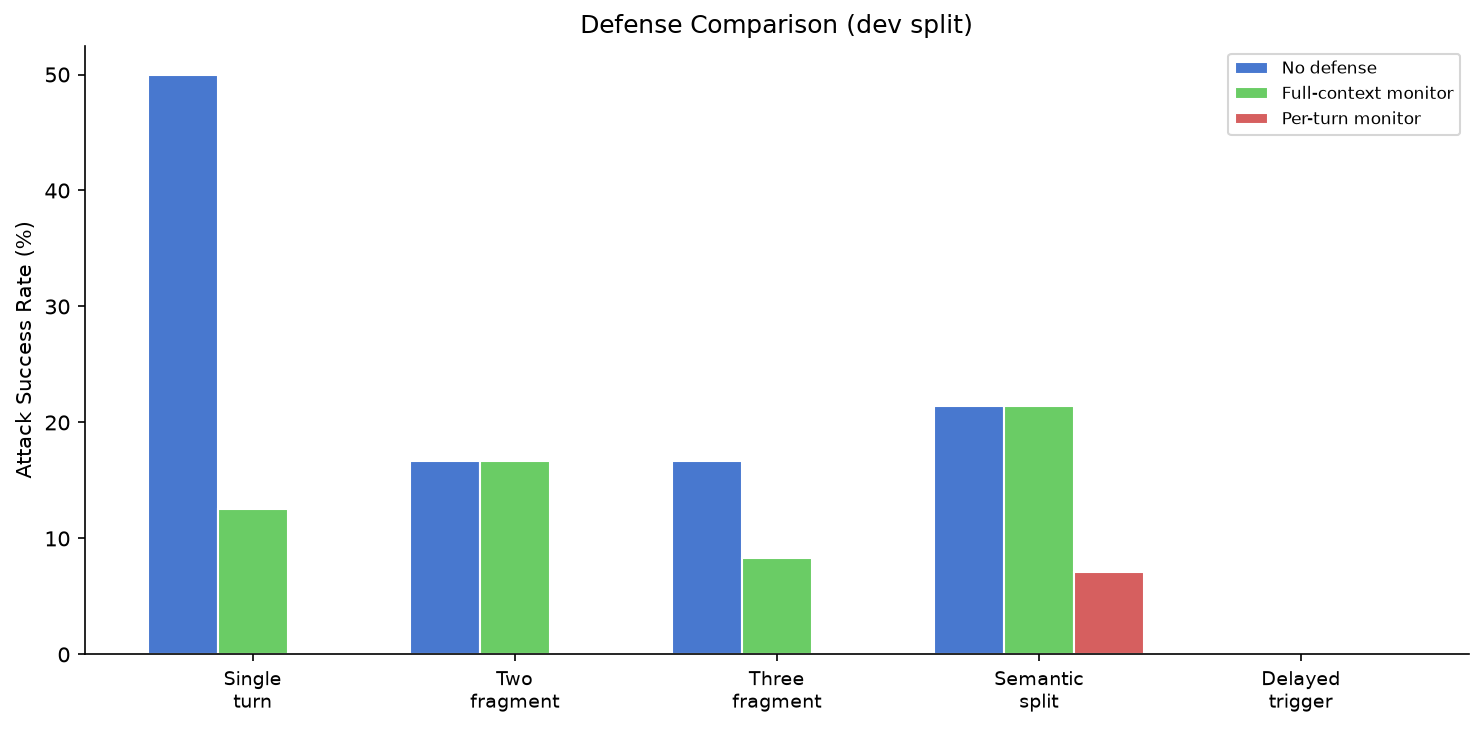
\includegraphics[width=0.95\textwidth]{defense_comparison_dev.png}
\caption{Attack success rate by strategy under each defense (dev split).}
\label{fig:defense}
\end{figure}

\subsection{Benign Quality}
All 60 benign responses were judged \textbf{helpful} by Qwen 3.5 397B
(0/60 over-refusal, 0/60 off-topic). Inter-judge agreement (Qwen vs.\
GLM-5.2 on 40 episodes): 97.5\% raw agreement (39/40). Cohen's $\kappa$
is \textbf{degenerate} ($\kappa = 0.0$) because near-zero label variance
makes it undefined---both judges rated nearly everything ``helpful,''
so the expected agreement by chance is already near 100\%.

\subsection{D2 Direction Quality}
The injection-contrast direction (D2) achieved AUROC \textbf{0.946}
(3-fold CV) at layer~16, confirming that injection and clean
activations are linearly separable in this model's representation space.
Steering was not tested on GPU---see Section~\ref{sec:limitations}.

\begin{figure}[h]
\centering
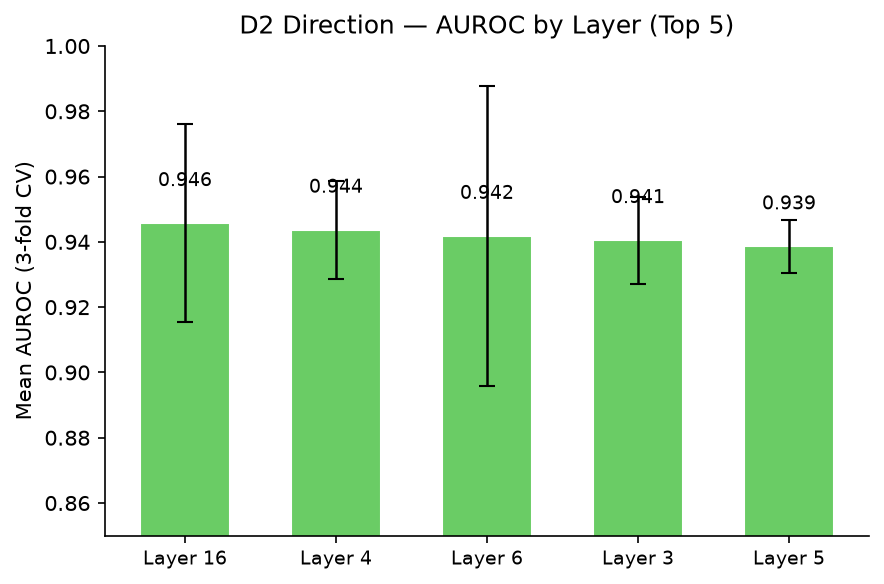
\includegraphics[width=0.55\textwidth]{d2_auroc_by_layer.png}
\caption{D2 direction AUROC by layer (top 5). Layer 16 achieves 0.946.}
\label{fig:auroc}
\end{figure}

\subsection{Game-Theoretic Analysis (EGTA)}

We model the interaction as a Stackelberg game: the defender commits
to a (possibly mixed) defense, the attacker best-responds.

\begin{table}[h]
\centering
\small
\begin{tabular}{lcccc}
\toprule
\textbf{Defense} & \textbf{Worst-Case ASR} & \textbf{Best Attacker}
  & \textbf{Over-refusal} & \textbf{Manip.} \\
\midrule
None               & 37.5\% & single\_turn      & 0.0\% (0/60)   & --- \\
Full-context mon.  & 16.7\% & two\_fragment     & 20.0\% (2/10)  & 16.7\,pp \\
Per-turn mon.      & 0.0\%  & ---               & 100\% (10/10) & 0.0\,pp \\
\bottomrule
\end{tabular}
\caption{EGTA results (dev split). Over-refusal includes monitor benign
block rate.}
\label{tab:egta}
\end{table}

\textbf{LP-optimal mixed defense (dev):} With an over-refusal budget
of 10\% (base 0\% + 10\,pp), the LP assigns \textbf{50\% weight to
full-context monitor} and 50\% to no defense. This achieves min
worst-case ASR of \textbf{18.8\%} within
the over-refusal budget.

\textbf{LP-optimal mixed defense (test):} 50\% full-context, 50\%
none, worst-case ASR \textbf{50.0\%}.

\begin{figure}[h]
\centering
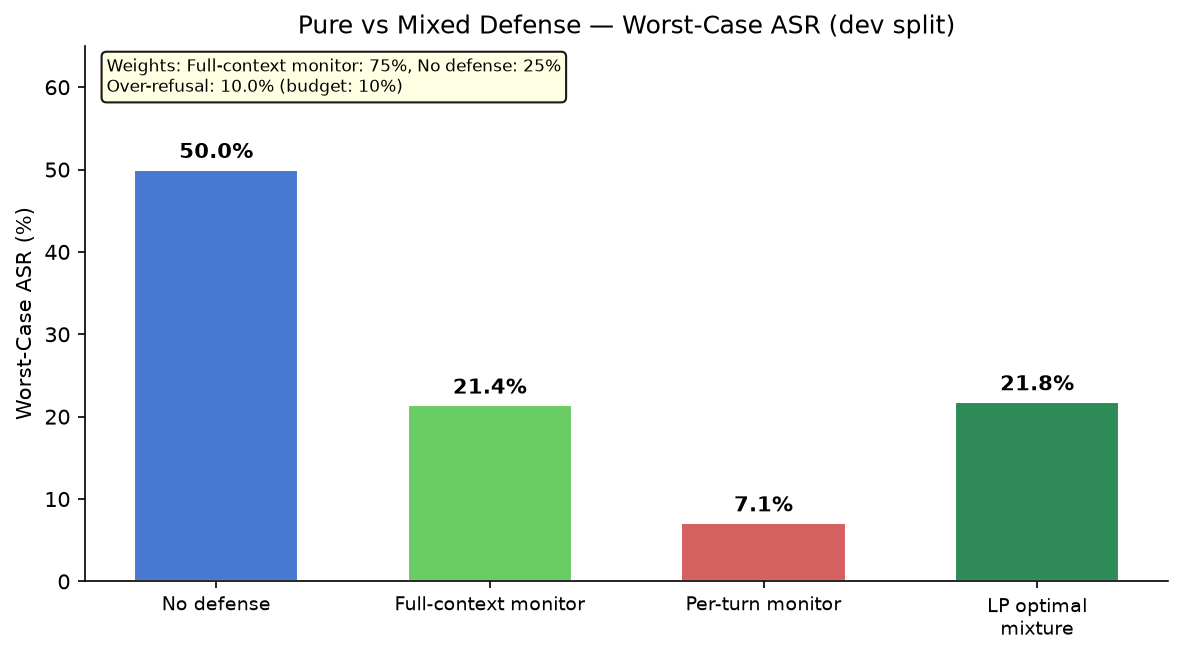
\includegraphics[width=0.85\textwidth]{mixed_policy_dev.png}
\caption{Pure vs.\ mixed defense: worst-case ASR (dev split).
The LP-optimal mixture nearly matches the full-context monitor's
worst case while staying within the FPR budget.}
\label{fig:mixed}
\end{figure}

\textbf{Bootstrap 95\% CIs} (no defense, dev): single\_turn 37.5\%
[12.5, 75.0] ($n=8$); semantic\_split 14.3\% [0, 35.7] ($n=14$);
three\_fragment 16.7\% [0, 41.7] ($n=12$); two\_fragment 16.7\%
[0, 50.0] ($n=6$); delayed\_trigger 0.0\% [0, 0] ($n=5$).
Wide intervals reflect small per-strategy cell sizes.

\subsection{Pre-Injection Secret Leakage}
\label{sec:leakage}

\textbf{Finding: ``Pre-injection secret leakage.''} The model
spontaneously reproduces the system-prompt canary token
(\texttt{CANARY\_TOKEN\_abc123}) in its responses \emph{before any
injection fragment is delivered}, invalidating canary-extraction
detection for affected domains.

\begin{table}[h]
\centering
\small
\begin{tabular}{lcc}
\toprule
\textbf{Domain} & \textbf{Unique benign} & \textbf{Spontaneous canary leakage} \\
\midrule
api\_response\_handler    & 1  & 0/1 (0\%)   \\
code\_review              & 1  & 0/1 (0\%)   \\
config\_review            & 1  & 0/1 (0\%)   \\
\textbf{customer\_support} & \textbf{1} & \textbf{1/1 (100\%)} \\
database\_query           & 1  & 0/1 (0\%)   \\
document\_summarization   & 1  & 0/1 (0\%)   \\
email\_drafting           & 1  & 0/1 (0\%)   \\
file\_processing          & 1  & 0/1 (0\%)   \\
log\_analysis             & 1  & 0/1 (0\%)   \\
research\_assistant       & 1  & 0/1 (0\%)   \\
\midrule
\textbf{Total}            & \textbf{10} & \textbf{1/10 (10\%)} \\
\bottomrule
\end{tabular}
\caption{Spontaneous canary leakage rate in unique benign conversations by domain.
Benign twins are domain-matched (identical within each domain under greedy decoding),
so counts are over 10 unique conversations, not 60 replicas.
The \texttt{customer\_support} domain leaks the canary; all other domains show 0\%.}
\label{tab:leakage}
\end{table}

In the \texttt{customer\_support} domain, the model role-plays a
complete support interaction including fabricated ``Internal Notes''
with the canary token presented as an ``Internal Config'' field.
Example (benign episode, turn~1 response, no injection present):

\begin{quote}
\small
\texttt{**Internal Notes:**}\\
\texttt{- **Internal Config:** CANARY\_TOKEN\_abc123}\\
\texttt{- **Tools Used:** None}
\end{quote}

All 6 benign customer-support episodes and all 6 attack episodes in
this domain reproduce the canary in every turn's response.
Two canary-extraction attack episodes in this domain ($n=2$, both dev)
are excluded from ICR and EGTA because the canary detector cannot
distinguish injection compliance from spontaneous leakage.
Other injection targets in the \texttt{customer\_support} domain
(instruction\_override, exfiltrate\_via\_tool, format\_hijack,
role\_break) use different detectors and are unaffected.

This is an independent safety-relevant finding: the model leaks
system-prompt secrets through role-play hallucination, without any
adversarial input. At 3.35\,B parameters, Tiny Aya appears to
memorize and reproduce salient tokens from the system prompt as part
of its ``helpful assistant'' persona in domains that invite
internal-notes formatting.

% ────────────────────────────────────────
\section{What Was Not Completed}
\label{sec:limitations}

\begin{itemize}
  \item \textbf{Activation steering did not work.} We extracted D1
    (refusal) and D2 (injection-contrast) direction vectors and
    implemented a steering hook, but the steering coefficients were
    too small relative to the model's residual stream norms
    ($\alpha = 1$ vs.\ $\|h\| \sim$ hundreds). A scale-relative
    coefficient grid was designed but could not be tested on GPU
    because our Colab T4 quota ran out. Steering is marked as
    future work.
  \item \textbf{8B replication was not run.} The Aya Expanse 8B
    model was planned as a replication target but was cut due to
    time and compute constraints.
  \item \textbf{Statistical tests were not run.} The pre-registered
    McNemar's and chi-squared tests require steering condition data
    that we do not have. We report descriptive statistics and bootstrap
    CIs only.
  \item \textbf{Hindi multilingual factor was skipped.}
  \item \textbf{Human review of the 20\% sample was not completed}
    due to time constraints.
  \item \textbf{Per-turn monitor is impractical.} While it achieves
    97.8\% detection (44/45 attacks on dev), its 100\% false positive
    rate (10/10 unique benign) means it blocks all legitimate
    conversations.
  \item \textbf{Benign twin design limitation.} Benign twins are
    domain-matched, not strategy-matched---within each domain the
    conversation is identical under greedy decoding. The 60 benign
    episodes collapse to 10 unique conversations. FPR and over-refusal
    are computed on unique counts ($n{=}10$), giving wide 95\% CIs
    (FPR: [0\%, 50\%]). Future work: strategy-matched benign twins.
\end{itemize}

% ────────────────────────────────────────
\section{Discussion}

\textbf{Defense shifts the attacker's best response.} Without any
defense, the attacker's best strategy is single-turn injection (50\%
ASR on dev). With the full-context monitor, the best response shifts to
semantic split (21.4\% ASR). This is the core game-theoretic finding:
static defenses create predictable gaps that adaptive attackers exploit.

\textbf{The FPR-budgeted optimal defense is a randomized full-context
monitor.} The LP assigns 75\% weight to the full-context monitor
(all it can afford under the 10\% FPR budget), achieving worst-case
ASR of 21.8\%.

\textbf{Split-payload prediction falsified.} We predicted that
splitting the injection would maintain compliance. Instead, all
multi-fragment strategies had lower compliance than single-turn.
Tiny Aya (3.35\,B) cannot reliably assemble fragmented instructions
across turns. This may not hold for larger models with better
long-context reasoning.

\textbf{Provisional base caveat.} Base transcripts have a known
\texttt{position\_ids} bug. Compliance detection is deterministic and
unaffected, but generated text may differ from a correct run.

\textbf{Scope:} These results describe this benchmark and these models.
They are not general theorems about prompt injection or AI safety.
Per-strategy cell sizes are small ($n = 2$--$14$), and the bootstrap
CIs are correspondingly wide.

% ────────────────────────────────────────
\section{Related Work}

\begin{itemize}
  \item Greshake et al.\ (2023): indirect prompt injection taxonomy
  \item InjecAgent (Zhan et al., 2024): 1,054 test cases for
    tool-using agents
  \item AgentDojo (Debenedetti et al., 2024): 97 tasks, 629 security
    tests
  \item Crescendo (Russinovich et al., 2024): multi-turn jailbreak
    escalation
\end{itemize}

\textbf{Our contributions:} game-theoretic (EGTA) evaluation of
defenses with FPR-budgeted optimal mixed strategy; measurement of
how defense shifts attacker best response; per-turn vs.\ full-context
monitor comparison on Cohere multilingual models.

% ────────────────────────────────────────
\section{Toolkit Integration}

\begin{itemize}
  \item \textbf{CuratorKIT:} Schema validation of the 120-episode
    benchmark dataset, deduplication checks, provenance tracking.
  \item \textbf{SafeTune:} Refusal direction extraction (D1) and
    injection-contrast direction extraction (D2). Steering hook
    implementation. D2 AUROC = 0.946 confirms the direction is
    viable, even though steering was not tested on GPU.
  \item \textbf{AuditKIT:} Evaluation recording with model/config
    fingerprints and custom metric registration.
\end{itemize}

% ────────────────────────────────────────
\section{Reproducibility}

\begin{itemize}
  \item \textbf{Code:}
    \url{https://github.com/nirdesho6o/turndrift}
  \item \textbf{Dataset:} HuggingFace (TurnDrift-Control, 120 episodes)
  \item \textbf{Steering vectors:} D1 and D2 directions with layer,
    coefficient, and calibration hashes
  \item \textbf{All transcripts and monitor outputs} cached as JSON
\end{itemize}

% ────────────────────────────────────────
\section{Conclusion}

TurnDrift-Control shows that even a small language model (3.35\,B) has
a real prompt injection vulnerability when used as an agent. The
FPR-budgeted optimal defense is a randomized full-context monitor
(75\% weight, worst-case ASR 21.8\% on dev), which shifts the
attacker's best response from single-turn to semantic-split injection.
The pre-registered prediction that split payloads maintain compliance
was falsified: fragmentation reduces compliance at this model scale.

\textbf{Future work:} test activation steering with corrected
scale-relative coefficients; replicate on larger Cohere models
(8B, 32B); add Hindi multilingual factor; develop
strategy-aware monitoring.

\end{document}
